%
%                       This is a LaTeX 2e version of the
%                       laboratory project template file.
\documentclass[a4paper,twoside,12pt]{article}
\usepackage{fullpage,epsf}
\usepackage{color,graphicx,natbib}
\usepackage{gensymb}
\graphicspath{ {C:/Users/Emma/Documents/TU Delft/International Course for Computational Physics} }

% Make subscripts in text available
\DeclareRobustCommand*\textsubscript[1]{%
  \@textsubscript{\selectfont#1}}
\def\@textsubscript#1{%
  {\m\ensuremath{_{\mbox{\fontsize\sf#1}}}}}
%
%                       This section generates a title page
%                       Edit only the sections indicated to put
%                       in the project title, your name, supervisor,
%                       project length in weeks and submission date
%
\begin{document}
\pagestyle{empty}                       							% 	No numbers of title page                      
                                           								% 	Centre Title, and name
\vspace*{2cm}
\begin{center}
        \Large\bf \Large\bf Report to assignment 1 \\
        \Large\bf International Course for Computational Physics\\[10pt]% 	Change to MP/CP/Astro
        \LARGE\bf Simulation of Argon particles in a box         		% 	Change to suit
\end{center}
\vspace*{0.5cm}
\begin{center}
        \bf Emma C. Gerritse, Sophie Hermans and Jason Emming\\ 	% 	Replace with your name
        March 2015                                    						%	Submission Date
\end{center}
\vspace*{5mm}
%
%                       Insert your abstract HERE
%                       
\begin{abstract}
This report describes the results of the simulation of Argon particles under the influence of a Lennard-Jones potential, using Python. Up to a 1000 particles have been simulated in a box with periodic boundary conditions. From the positions, momenta and forces of all of the particles the total, potential and kinetic energies, the temperature, pressure and correlation function for the system and their corresponding errors have been calculated.
\end{abstract}

\vspace*{2cm}
Signature:\hspace*{8cm}Date:

\vfill
{\bf Lecturers:} Dr. Jos Thijssen and Dr. Phil Duxbury        	% 	Change to suit
\hfill
\textbf{Year:} 2014-2015                 					% 	Change to suit
\newpage
											%      End of Title Page
\pagestyle{plain}                               					% 	Page numbers at bottom
\setcounter{page}{1}                         					% 	Set page number to 1
\tableofcontents                                					% 	Makes Table of Contents

\pagebreak


\section{Introduction}
\noindent How particles in a system move and interact is what molecular dynamics strives \mbox{to answer.} Developing a computer simulation to accurately predict the behavior of matter has applications that are wide and far reaching. From answering how galaxies evolve to precisely modeling the folding of amino acids into complicated proteins, each system must \mbox{involve} many particles. The motion of these particles is characterized by their potential, which governs the force between them. It was the mission of this group to simulate the consequences of the potential between individual atoms of Argon gas. 


\section{Theory}
\noindent In order to simulate a number of particles in a box, one first has to define a particle. The Argon atoms, in this case, have been modeled as point particles that have three properties: a position, a momentum and a potential.

\subsection{Potential and force}
\noindent The Argon particles exert a certain force on one another. They are net neutral particles, so it is a Lennard-Jones force that must be applied. This force can be derived from the Lennard-Jones potential given in equation \ref{eq:Vlenjon}.

\begin{equation}
\label{eq:Vlenjon}
V_{LJ} = 4\epsilon \left(\left(\frac{\sigma}{r}\right)^{12}-\left(\frac{\sigma}{r}\right)^6\right)
\end{equation}

\noindent In this equation, the potential has both a long range attractive component as well as a short range repulsive one. \textit{r} represents the distance between the two particles in question. The $\epsilon$ characterizes the strength of these interactions, while the  $\sigma$ defines the radius of an Argon particle and sets the range. The derivative of this potential then gives us the Lennard-Jones force, as shown in equation \ref{eq:Flenjon}.

\begin{equation}
\label{eq:Flenjon}
\hat{F}_{LJ} = 24\epsilon \left(\frac{\sigma^6}{r^7_{ij}}-2\frac{\sigma^{12}}{r^{13}_{ij}}\right)\hat{r}_{ij}
\end{equation}

\noindent Integrating the force for each particle and solving for its motion, we were able to simulate the movement of an N-body system of particles in a box.

\subsection{Extracting physical parameters}

\noindent Using our molecular dynamics model we observed the behavior of Argon particles as a function of their temperature. To determine the temperature we use the relationship between the velocities of the particles and their kinetic energy. This relation is given by the Maxwell-Boltzmann distribution in equation \ref{eq:Maxwell-Boltzmann}.

\begin{equation}
\label{eq:Maxwell-Boltzmann}
\frac{3}{2}(N-1)k_{B}T = \frac{1}{2}\sum_{i}m_{i}|\hat{v_{i}}^2|
\end{equation}

\noindent We also determined the density of particles from a particular point as a function of distance, known as a pair correlation function. To do this, we counted the number of particles that fell within a shell of radius r and shell width of $\delta$\textit{r}. With is, we plotted a histogram of the particle locations, see figures \ref{fig:cor_gas}, \ref{fig:cor_liquid}, \ref{fig:cor_solid}.
\vspace{5mm}

\noindent Finally, we calculated the pressure of the particles in this volume, which follows from the virial relation given in equation \ref{eq:virial}. 

\begin{equation}
\label{eq:virial}
pV = Nk_{B}T+\frac{1}{3}\sum_{i<j}\hat{r_{ij}}\cdot\hat{F_{ij}}
\end{equation}


\section{Computational theory}

\noindent To simulate the problem of Argon particles in a 3D box, we have made a code in Python. Next to the theory of the needed physics, we also need some theory about the computational part, such as boundary conditions, see section \ref{sec:boun}, and initial conditions, section \ref{sec:ini}.

\subsection{Boundary conditions}\label{sec:boun}

\noindent In our molecular dynamics code we implemented periodic boundary conditions. By doing so, we approximated a seemingly infinite system, while only simulating a small unit of the whole. As particles moved outside the boundary they re-emerged on the other side of the box, while still maintaining their momentum.
The positions of the Argon atoms were checked every iteration of the program. If they had wandered beyond the length of the box, $L$, the modulo of their position, $\vec{x}$, was taken. This moved them to an appropriate position within the boundary conditions i.e. $\vec{x}_{new}=\vec{x} \bmod L$
\vspace{5mm}

\noindent The boundary conditions were also taken into account for the potential calculations. We had to determine the shortest distance from one particle to another in order to accurately gauge its magnitude. This must allow for distances to be measured through the edges of the box as well. This prevented any particle from suddenly feeling a strong increase in force, which had not been present before, when it moved across the boundary.

\subsection{Initial Conditions}\label{sec:ini}

\noindent When the molecular dynamics simulation is running, the old positions, momenta and forces are used for every subsequent iteration, as described in section \ref{sec:verlet}. For the first calculation however, some initial values are needed. If these initial conditions are chosen randomly, the programme may never converge to a physical solution. Therefore, we have to set our initial conditions carefully.

\subsubsection{Initial Positions}

\noindent As an initial condition for the positions of the particles we used a face centered crystal (FCC) lattice, see figures \ref{fig:ini_pos_4} and \ref{fig:ini_pos_500}. One unit cell contains 4 particles located at $(0,0,0), (\frac{1}{2},\frac{1}{2},0), (\frac{1}{2},0,\frac{1}{2})$ and $(0,\frac{1}{2},\frac{1}{2})$.

\begin{figure}[h]
\centering
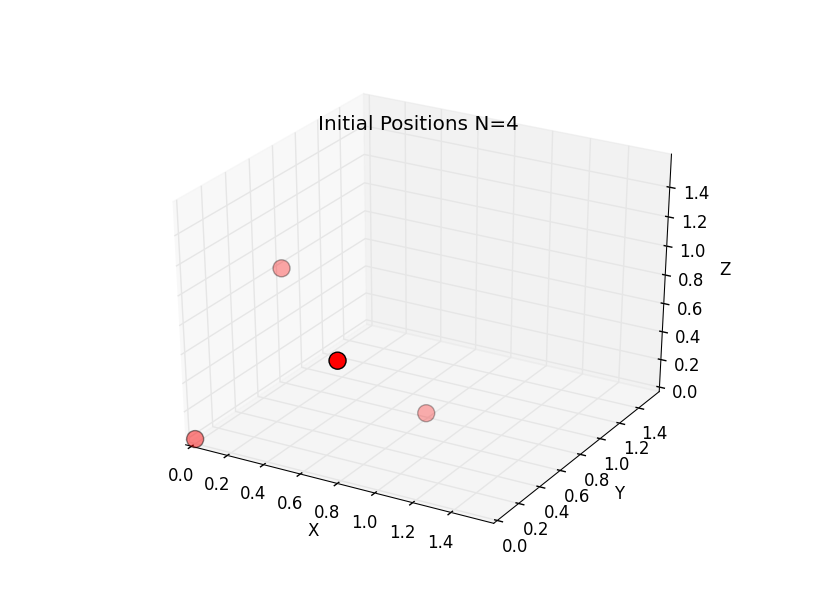
\includegraphics[scale=0.4]{figures/initial_positions_4.png}
\caption{A FCC lattice as initial positions for 4 particles.}
\label{fig:ini_pos_4}
\end{figure} 

\begin{figure}[h]
\centering
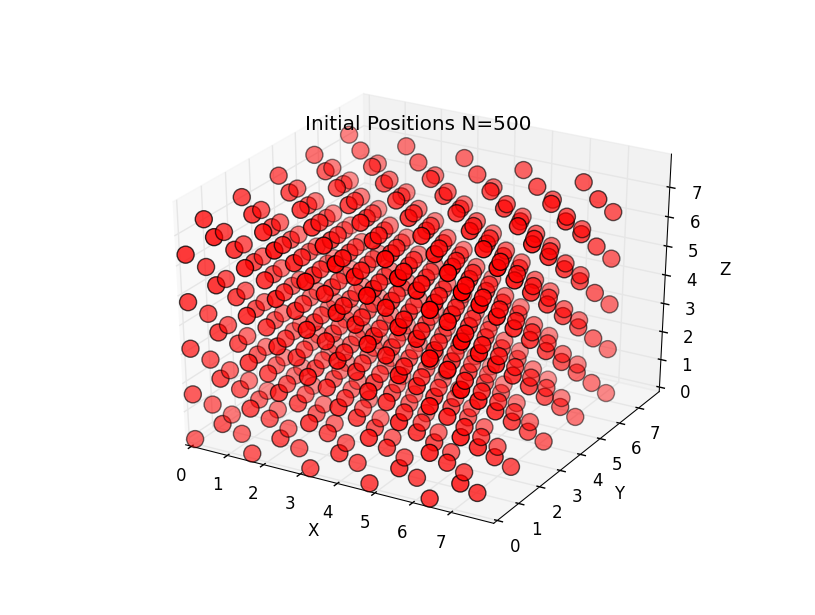
\includegraphics[scale=0.4]{figures/initial_positions_500.png}
\caption{A FCC lattice as initial positions for 500 particles.}
\label{fig:ini_pos_500}
\end{figure} 

\subsubsection{Initial Momenta}

\noindent The initial momenta have been generated using a Gaussian distribution in the x-, y-, and z-direction, with $\mu=0$ and $\sigma^{2}=2T$. This ensures a realistic physical distribution of the velocities. The zero mean gives a total momentum of exactly zero, if an infinite number of particles were to be simulated. Since we do not have an infinite number of particles, the average $\mu$ will never be exactly zero. Therefore we have to correct the momenta of all the particles in three dimensions by subtracting $\frac{1}{N}\sum_{i=1}^{N} p_{i}$, such that the average is equal to zero exactly. 

\begin{figure}
\centering
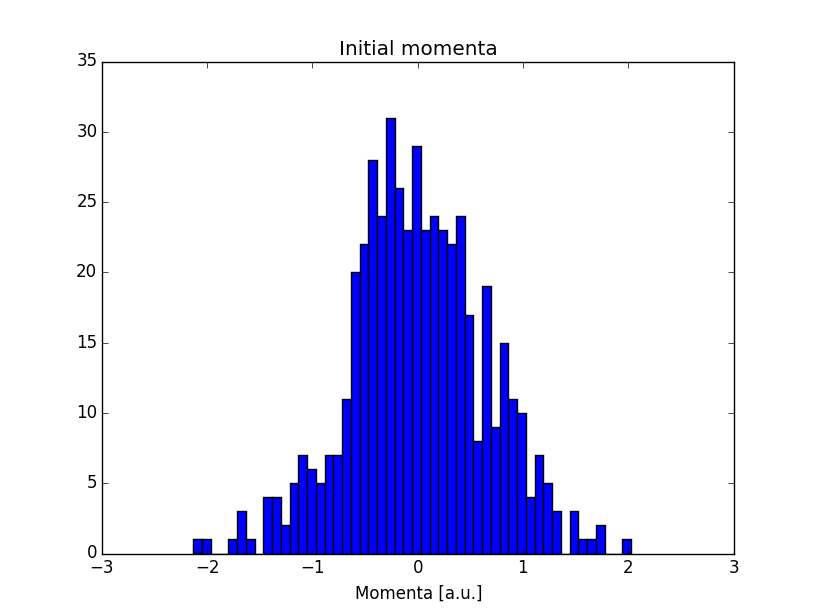
\includegraphics[scale=0.6]{figures/initial_momenta_500.png}
\label{fig:ini_mom_500}
\caption{A histogram of the initial momenta for 500 particles. It follows a Gaussian distribution with $\mu=0$ and $\sigma^{2}=2T$.}
\end{figure}

\subsection{Cut-off radius}

\noindent When two particles are far apart, their force on each other is very small, therefore their contribution to the total force can be neglected. In our code we have defined a cut-off radius. When the distance between two particles is larger than this radius, we do not calculate the contributing force, but simply set it to zero to save computation time. 

\subsection{Verlet's Theorem}\label{sec:verlet}

The positions of the particles are updated each iteration step. This can be done with simple Newtonian physics.

\begin{equation}
\vec{p} =\vec{p_0}+\vec{F}\Delta t 
\end{equation}
\begin{equation}
\vec{x}=\vec{x_0}+\vec{v_0}\Delta t
\end{equation}

\noindent Where $\vec{F}$ is the force coming from the Lennard Potential between the particles, which is also updated each iteration step. In this simulation program the mass of the particles is set to 1, so $\vec{p}=\vec{v}$ .
\vspace{5mm}

\noindent It turns out that this a rather crude approach, the positions and the momenta of the particles are only updated at integer time steps. A 'leapfrog' method such as the Verlet's Theorem would be more accurate, because this method uses the central difference for the velocity:

\begin{equation}
\vec{v}=\frac{d\vec{x}}{dt}=\frac{\vec{x}(t+\Delta t)-\vec{x}(t-\Delta t)}{2\Delta t} +O^{2}(\Delta t)
\end{equation}

\noindent The computational error is now of the second order, compared to a first order error in the case of a backward  or forward difference. 

\noindent So we have used the Verlet's Theorem in our programme:
\begin{equation}
\vec{p} = \vec{p_0}+\frac{1}{2}\vec{F}\Delta t
\end{equation}
\begin{equation}
\vec{x}=\vec{x_0}+\vec{v_0}\Delta t
\end{equation}
\begin{equation}
\vec{F}=\sum_{i,j}\vec{F}(\vec{x_i}-\vec{x_j})
\end{equation}
\begin{equation}
\vec{p} = \vec{p}+\frac{1}{2}\vec{F}\Delta t
\end{equation}

\subsection{Data blocking}\label{sec:data}

The most straight forward way to calculate the error in computationally simulated data, is to take use the central limit theory in calculating a mean and a standard deviation from that mean. However, this only works for uncorrelated samples. In reality, the data are often showing some memory, as is the case in Molecular Dynamics simulations. All the data within a range $\tau$ of a data point are correlated to that data point. If the time-step between data points $\Delta t$ is smaller than $\tau$, we can use a method called \textit{data blocking}.
\vspace{5mm}

\noindent When using data blocking, the sample of data points is divided into subsequent data blocks. These blocks are of such size that the $n^{th}$ data point of block $i$ is not correlated with the $n^{th}$ data point of block $i+1$. The minimal size satisfying this condition is the correlation time $\tau$, and this is most commonly used as the block size. In order to get this $\tau$, an autocorrelation function of the data is determined. The correlation time $\tau$ is the time at which the correlation drops below half of the autocorrelation at zero. For the error, we then use equation \ref{eq:error} where $\sigma$ is the standard deviation and M the total number of data points.

\begin{equation}
e = \sqrt{\frac{2\tau}{M}}\sigma
\label{eq:error}
\end{equation}

\subsection{Temperature renormalization}\label{sec:tem}

\noindent In physical experiments, often the temperature of the system is held at a fixed value. In order to simulate this our programme we keep the temperature fixed as an input parameter by using a temperature renormalization.
In other words we want to assign a specific value to the kinetic energy. We do this by adjusting the momenta of the particles.

\begin{equation}
v'= \sqrt{\frac{T_{target}}{T}}v
\end{equation}

\noindent Where $T_{target}$ is the temperature you want to maintain and $T$ the actual temperature in the system. 


\section{Results}

\subsection{Energy}

\noindent The total energy of the system is defined by equation \ref{eq:energy}.

\begin{equation}
E_{tot}=E_{pot}+E_{kin}
\label{eq:energy}
\end{equation}

\noindent The total energy should be conserved for all the time steps. The results for this is plotted in figure \ref{fig:energy}.

\begin{figure}[h]
\centering
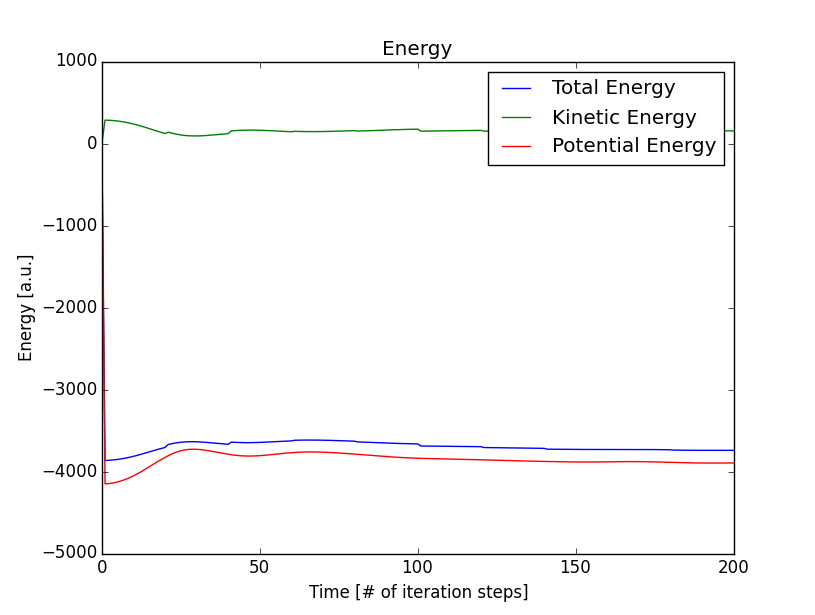
\includegraphics[scale=0.5]{figures/Energies_500}
\caption{The total, potential and kinetic energies plotted for different time steps.}
\label{fig:energy}
\end{figure}

\begin{table}
\centering
\caption{Overview of the mean values and errors of the energy of the system for 500 particles and 200 time steps.}
\begin{tabular}{|l|r|r|}
\hline
 & Mean value [a.u.] & Error [a.u.] \\
 \hline
Total Energy & -3679.1 & 26.6  \\
Potential Energy & -3834.7 & 28.2 \\
Kinetic Energy & 155.58 & 4.73 \\
\hline
\end{tabular}
\label{tab:energy}
\end{table}

\subsection{Temperature}

\noindent As described in section \ref{sec:tem}, the temperature can be held constant using a temperature renormalization algorithm. The results for 500 particles and 200 time steps are plotted in figures \ref{fig:tem_ren} and \ref{fig:tem} for with and without temperature renormalization respectively.
\vspace{5mm}

\begin{figure}[h]
\centering
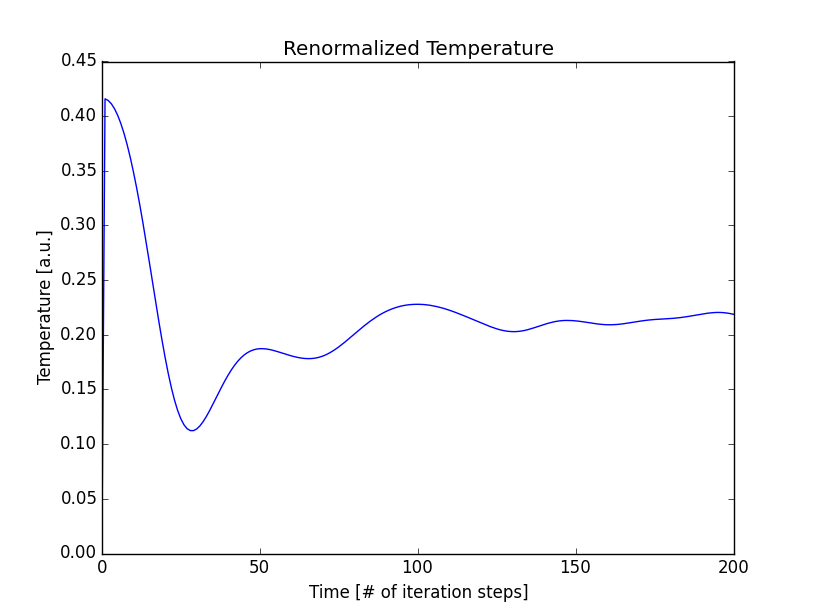
\includegraphics[scale=0.5]{figures/temperature_500.png}
\caption{Temperature of the system with 500 particles for 200 time steps, without renormalization.}
\label{fig:tem}
\end{figure}

\begin{figure}[h]
\centering
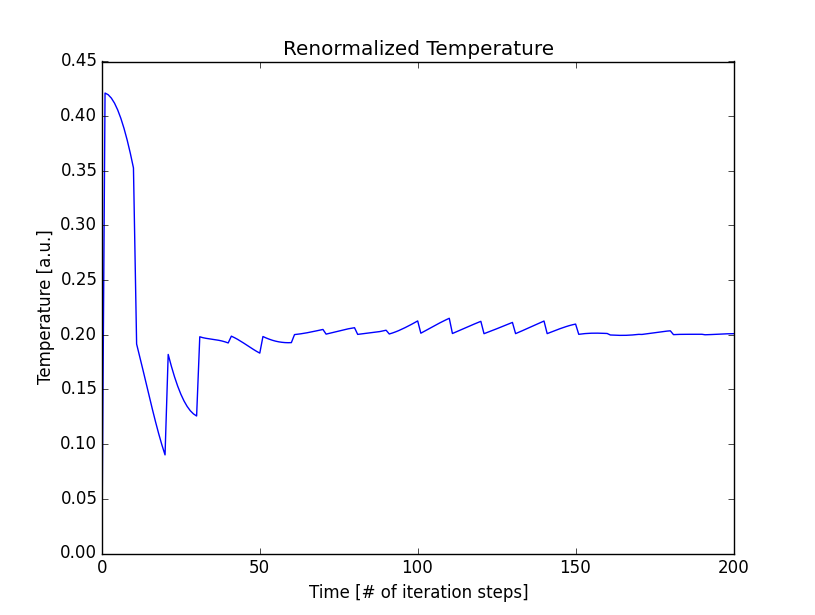
\includegraphics[scale=0.5]{figures/temperatures_renormalized_500.png}
\caption{Temperature of the system with 500 particles for 200 time steps, with renormalization.}
\label{fig:tem_ren}
\end{figure}

\noindent We have also calculated the average temperature with and without renormalization and the corresponding errors using the method described in section \ref{sec:data}. The results are shown in table \ref{tab:tem}.

\begin{table}
\centering
\caption{Overview of the mean values and errors of the temperature of the system for 500 particles and 200 time steps.}
\begin{tabular}{|l|r|r|}
\hline
 & Mean value [a.u.] & Error [a.u.] \\
 \hline
Temperature & 0.210 & 0.011  \\
Temperature (renormalized) & 0.2048 & 0.0071 \\
\hline
\end{tabular}
\label{tab:tem}
\end{table}

\subsection{Pressure}

\noindent We have calculated the pressure according to equation \ref{eq:virial} for 500 particles and a temperature of $T= 0.2$ in arbitrary units, see figure \ref{fig:pres}. We have computed the average value and its error, see table \ref{tab:pres}.

\begin{figure}[h]
\centering
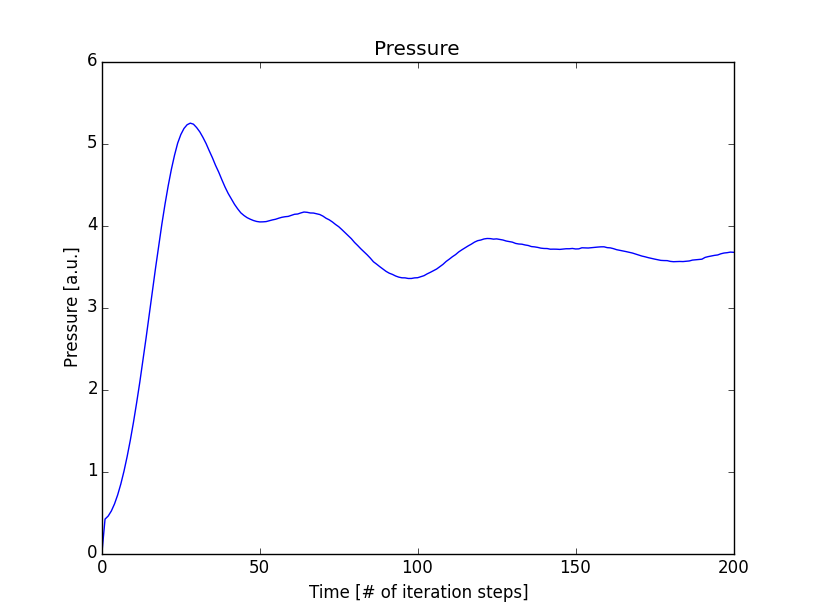
\includegraphics[scale=0.5]{figures/pressure_500.png}
\caption{ The pressure in the system for 500 particles and a temperature of $T=0.2$ [a.u.].}
\label{fig:pres}
\end{figure} 

\begin{table}
\centering
\caption{Mean value and error of the pressure in the system for 500 particles and 200 time steps.}
\begin{tabular}{|l|r|r|}
\hline
 & Mean value [a.u.] & Error [a.u.] \\
 \hline
Pressure & 3.67 & 0.21 \\
\hline
\end{tabular}
\label{tab:pres}
\end{table}

\subsection{Correlation function}

\noindent With our programme we have computed the correlation function for three different states of the system; gas, liquid and solid. The results are plotted in figures \ref{fig:cor_gas}, \ref{fig:cor_liquid} and \ref{fig:cor_solid} respectively. The different states are obtained by changing the (renormalized) temperature.

\begin{figure}
\centering
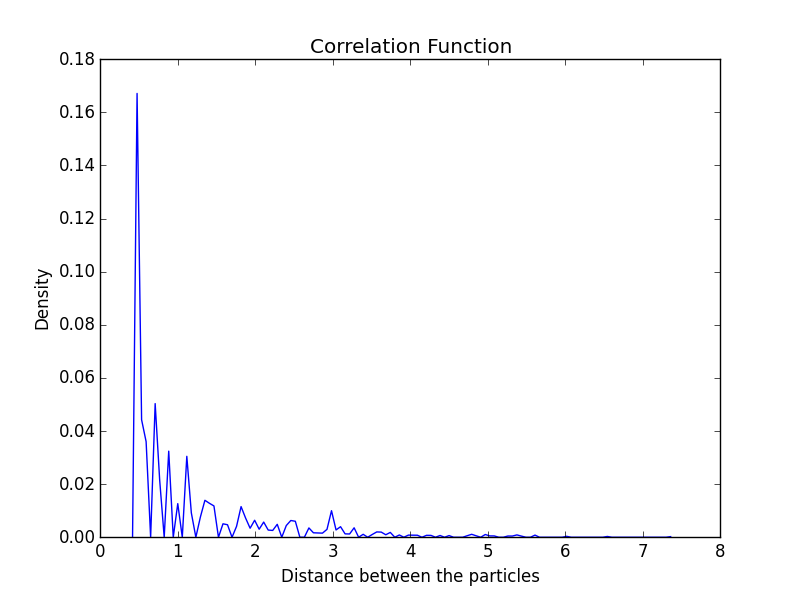
\includegraphics[scale=0.6]{figures/Corr_func_gas_2.png}
\caption{Correlation function of the gas state of the system with 108 particles for a temperature $T=2$ [a.u.].}
\label{fig:cor_gas}
\end{figure}

\begin{figure}
\centering
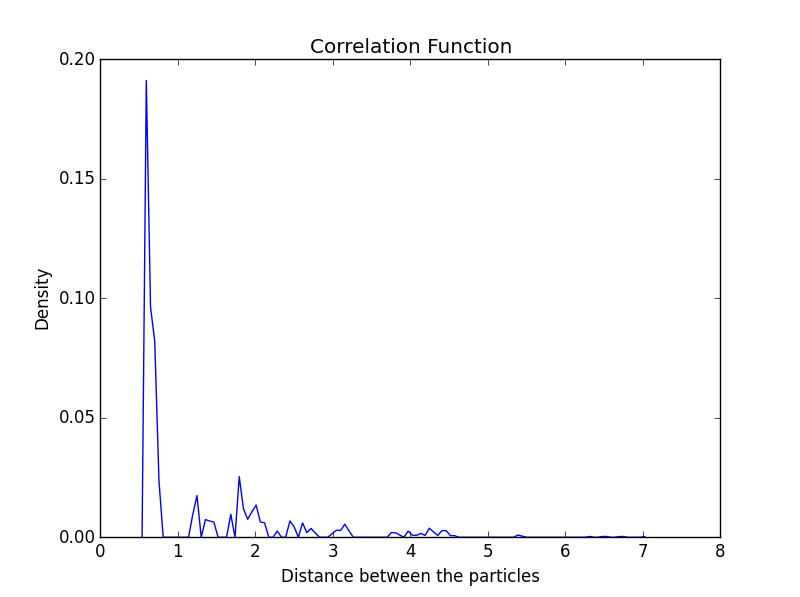
\includegraphics[scale=0.6]{figures/Corr_func_liquid_2e-4.png}
\caption{Correlation function of the liquid state of the system with 108 particles for a temperature $T=2 \cdot 10^{-4}$ [a.u.].}
\label{fig:cor_liquid}
\end{figure}

\begin{figure}
\centering
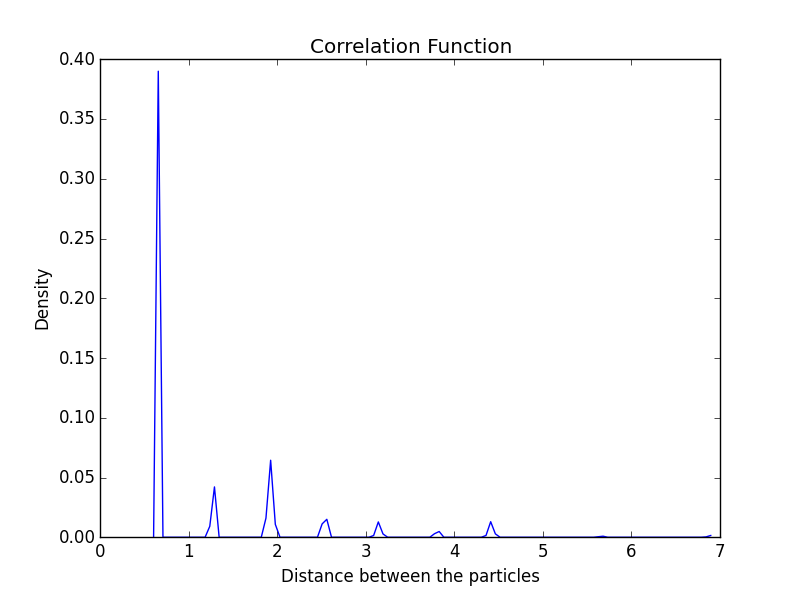
\includegraphics[scale=0.6]{figures/Corr_func_solid_2e-6.png}
\caption{Correlation function of the solid state of the system with 108 particles for a temperature $T=2 \cdot 10^{-6}$ [a.u.].}
\label{fig:cor_solid}
\end{figure}

\subsection{Computation Time}
\noindent To see how our programme handles a larger number of particles, we have measured the computation time for different number of particles/unit cells. The results can be seen in figures \ref{fig:comp_A} and \ref{fig:comp_N}. We noticed that the first step takes a lot more time than the others, because it has to initialize the problem, i.e. the initial momenta and positions. That is the reason we have the computation time for 1 and 11 time steps. 

\begin{figure}
\centering
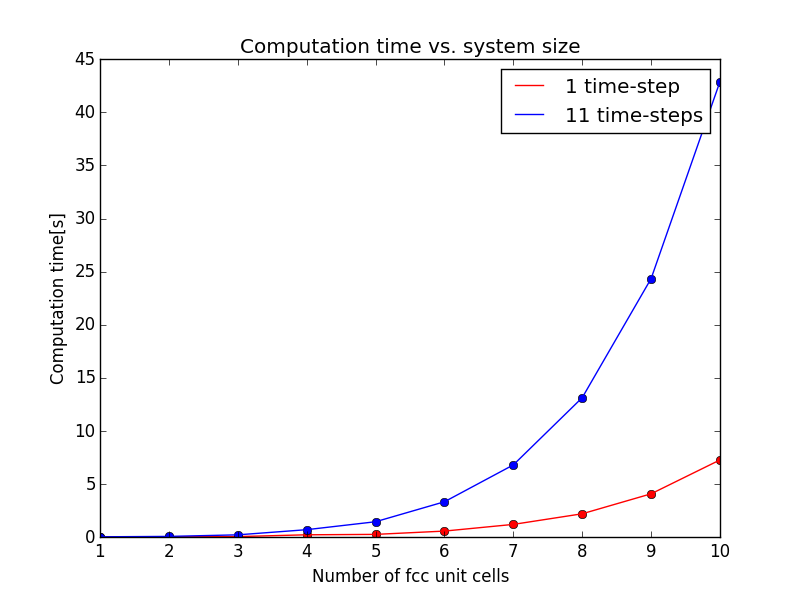
\includegraphics[scale=0.6]{figures/computationtime_unitcells}
\caption{Computation time in seconds for an increasing number of unit cells.}
\label{fig:comp_A}
\end{figure}

\begin{figure}
\centering
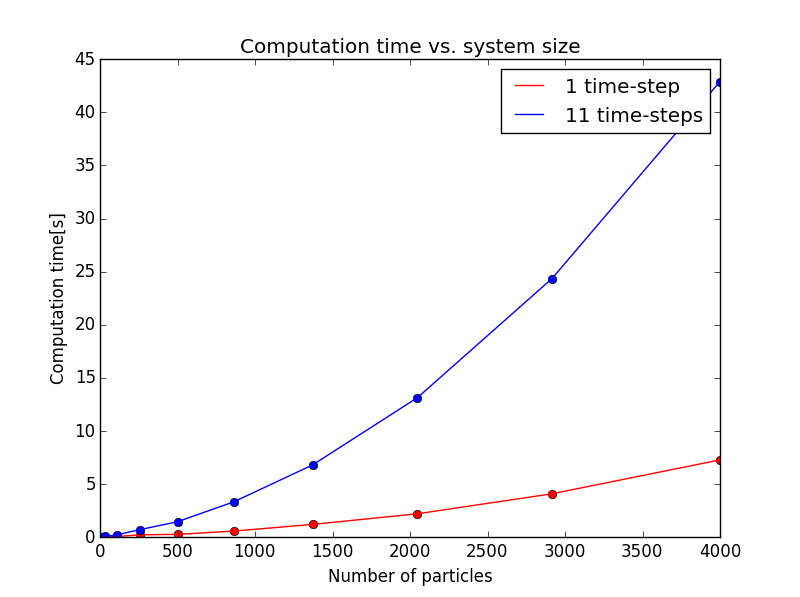
\includegraphics[scale=0.6]{figures/computationtime_particles}
\caption{Computation time in seconds for an increasing number of particles.}
\label{fig:comp_N}
\end{figure}

\subsection{Animation}

\noindent We were able to keep track of each particle?s positions following every iteration run and use this data to animate its motion in real time. We did this by plotting the x,y,z coordinates of each Argon atom on a 3D scatter plot. We continually updated its positions, while erasing the previous one. This gave the illusion of motion as the program ran. 
\vspace{5mm}

\noindent By varying the temperature in the initial conditions we formed Argon in both a solid and gaseous states, see figures \ref{fig:Ani_solid} and \ref{fig:Ani_gas}.

\begin{figure}
\centering
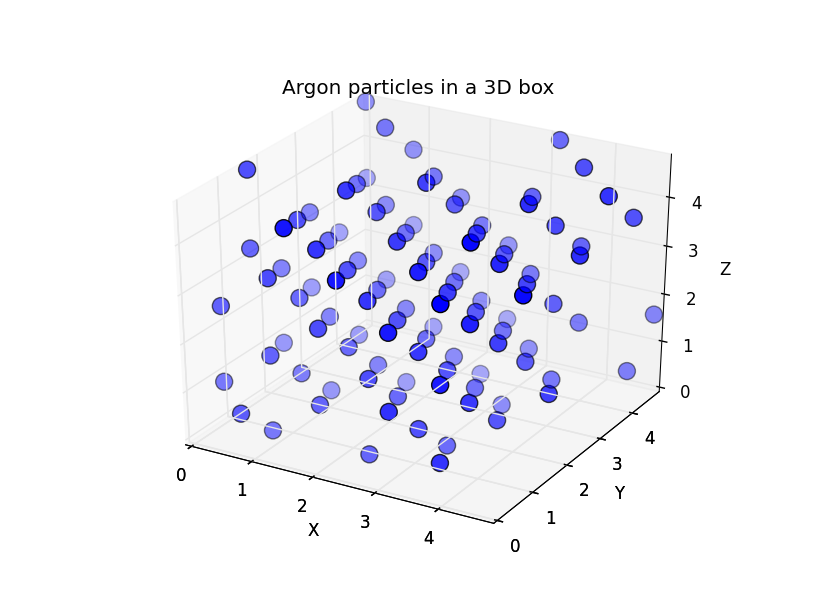
\includegraphics[scale=0.6]{figures/ani_solid_2e-6.png}
\caption{Animation solid}
\label{fig:Ani_solid}
\end{figure}

\begin{figure}
\centering
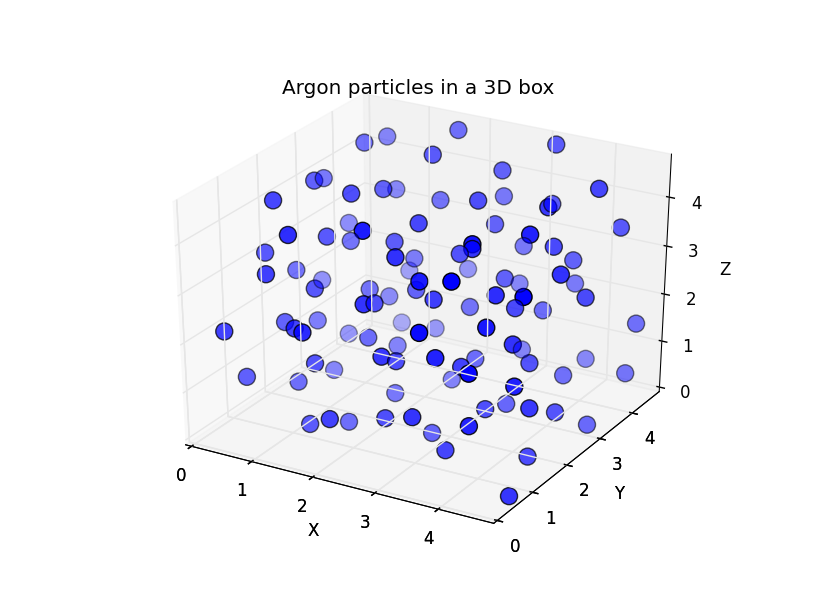
\includegraphics[scale=0.6]{figures/ani_gas_2.png}
\caption{Animation gas}
\label{fig:Ani_gas}
\end{figure}

\begin{figure}
\centering
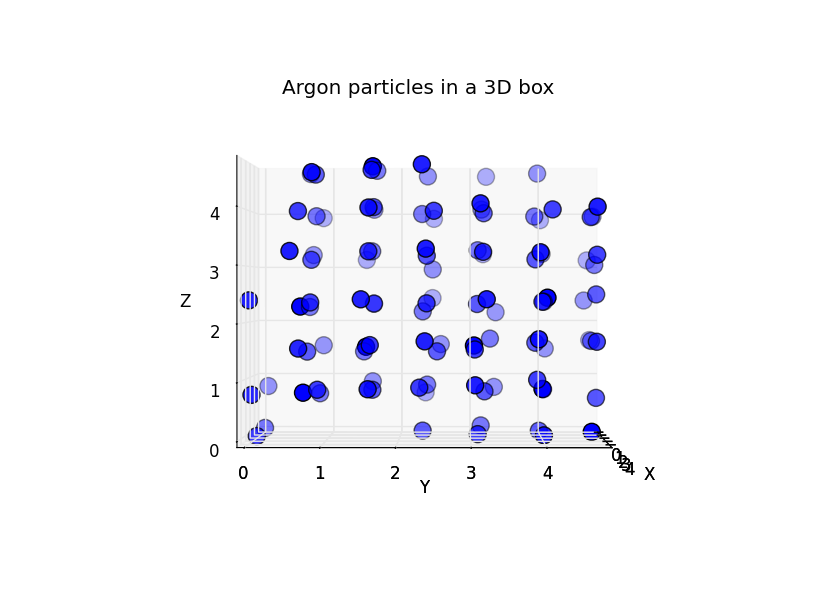
\includegraphics[scale=0.6]{figures/ani_wiggle.png}
\caption{Animation gas wiggle}
\label{Animation_gas_wiggle}
\end{figure}
\newpage

\section{Conclusions and Discussion}

\noindent The Python-based molecular dynamics simulation described in this report can simulate at least 500 Argon particles in a box with periodic boundary conditions. This program has functionalities to fix or get the temperature, calculate the pressure and the correlation function, and animate the movement of the Argon particles in a visually appealing manner. During these simulations, the energy and momentum in the system are conserved to a reasonable degree.
\vspace{5mm}

\noindent Improvements on this program could be made by increasing the efficiency of the code, for example, exporting portions to Fortran to execute the time-consuming parts of the calculation, such as the force and distance calculations. Another improvement would be the extension of functionalities, like a heat capacity calculation module. A third improvement builds upon an assumption made at the beginning of the program, which is that all physical constants (the Boltzmann factor, the unit cell size, etc.) are unity. Implementing the correct physical values would make for easier use of the program, by enabling the user to input familiar values for the box length, temperature, pressure and other input parameters.
\vspace{5mm}

\noindent In the end, the simulation of Argon particles using this simulation is a useful exercise to gain more insight into the physical properties an intricacies of such an apparently simple system. It can visually show the difference of particle behavior in different phases of matter (solid, liquid and fluid).

\end{document}











